\section{Week 9}
\Large \textbf{{\color{red}\underline{Mixure}}}

\begin{enumerate}
    \item \textbf{\ul{Compressibility factor}}
    \begin{itemize}
        \item Ideal gas: 
        \begin{equation*}
            Pv = RT
        \end{equation*}
        Assumptions made:
        \begin{itemize}
            \item particles of zero size/volume
            \item no attractive forces
            \item perfectly elastic collisions
        \end{itemize}
        Hold for {\color{green}low pressure high temperature gases} but not for {\color{red}gases in engine/power reactors}. Gases behave ideally when $T_R > 2$ regardless of pressure except when $P_R >> 1$.
        \item 'Compressed' ideal gas:
        \begin{align*}
            Pv &= {\color{blue}Z}RT\\
            \text{where } {\color{blue}Z} &= \frac{v_{actual}}{v_{ideal}}, \\
            {\color{blue}Z} &= \begin{cases} 
            >1, \\
            =1, \\
            < 1
            \end{cases}
        \end{align*}
        \item {{\color{blue}Principle of Corresponding States}}
        \begin{itemize}
            \item {\color{blue}Reduced Pressure $P_r$}:
            \begin{equation*}
                P_r = \frac{P}{P_{cr}}
            \end{equation*}
            \item {\color{blue}Reduced Pressure $T_r$}:
            \begin{equation*}
                T_r = \frac{T}{T_{cr}}
            \end{equation*}
        \end{itemize}
        Gases behave similarly at T and P normalized wrp. to their critical $P_{cr}$ and $T_{cr}$.
    \end{itemize}
\begin{figure}[H]
    \centering
    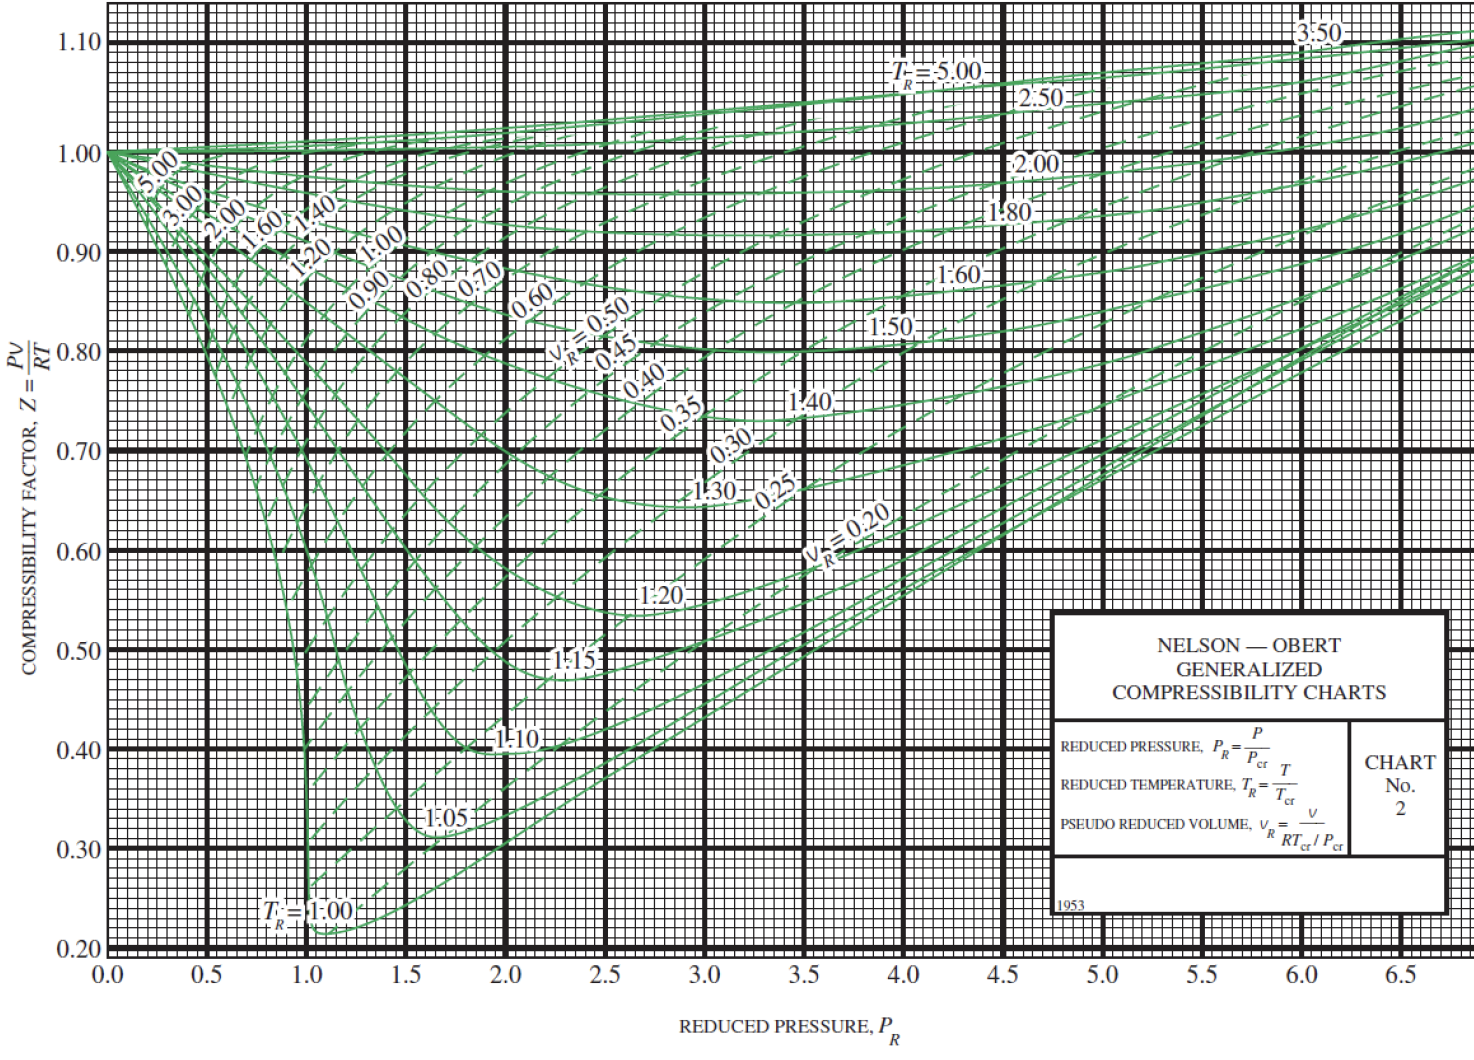
\includegraphics[width=1.0\linewidth]{images/Generalized_Compressibility_Chart.png}
\end{figure}
    \item \textbf{\ul{Van der Waals Equation of State (EOS):}}
    \begin{align*}
        \left(P+\frac{a}{v^2}\right)\cdot \left( v-b \right) &= RT \\
        a &= \frac{27\cdot R^2 T_{cr}^2}{64 \cdot P_{cr}} , \\
        b &= \frac{RT_{cr}}{8 \cdot P_{cr}}
    \end{align*}
    factor $a$ accounts for the inter-molecular forces; factor $b$ accounts for the volume taken up by molecues.
    \item \textbf{\ul{Pseudo-reduced volume}}
    \begin{equation*}
        v_r = \frac{v}{\frac{RT_{cr}}{P_{cr}}}
    \end{equation*}
\end{enumerate}

\Large \textbf{{\color{red}\underline{Ideal Gas Mixture}}}

\begin{itemize}
    \item Mass of mixture:
    \begin{equation*}
        m_m = \sum_{i=1}^{k} m_i
    \end{equation*}
    \item Number of moles in a mixture
    \begin{equation*}
        N_m = \sum_{i=1}^{k} N_i
    \end{equation*}
    \item Mass fraction
    \begin{equation*}
        m_{fi} = \frac{m_i}{m_m}
    \end{equation*}
    \item Mole fraction
    \begin{equation*}
        y_i = \frac{N_i}{N_m}
    \end{equation*}
    \item For all mixtures, it holds that:
    \begin{align*}
        \sum_{i=1}^{k} m_{fi} &= 1 \\
        \sum_{i=1}^{k} y_i &= 1 
    \end{align*}
    \item {\color{blue}The mass of a substance, $m$,} can be expressed in terms of the {\color{blue}mole number, $N$} and {\color{blue}molar mass, $M$} of the substance as {\color{blue}$m=N\times M$}. 
    \item The {\color{blue}apparent/average molar mass of a mixture} is defined as,
    \begin{align*}
        M_m &= \frac{m_m}{N_m}\\
        &=\frac{\sum m_i}{N_m} \\
        &= \frac{\sum N_i \cdot M_i}{N_m} \\
        &= \sum_{i=1}^{k} y_i M_i
    \end{align*}
    alternatively, as
    \begin{align*}
        M_m &= \frac{m_m}{N_m}\\
        &=\frac{m_m}{\sum m_i / M_i}\\ 
        &= \frac{1}{\sum m_i / (m_m M_i)}\\
        &= \frac{1}{\sum \frac{m_{fi}}{M_i}}
    \end{align*}
    \item Specific gas constant of a gas mixture:
    \begin{equation*}
        R_m = \frac{R_u}{M_m}
    \end{equation*}
    \item Mass and mole fractions are related by
    \begin{align*}
        m_{fi} &= \frac{m_i}{m_m} \\
        &= \frac{N_i M_i}{N_m M_m} \\
        &= y_i \frac{M_i}{M_m}
    \end{align*}
\end{itemize}

\Large \textbf{{\color{red}\underline{Dalton/Amagat's Laws}}}

\begin{itemize}
    \item {\color{blue}Dalton's Law of Additive Pressures:} the {\color{red}pressure of a gas mixture} is {\color{red}equal} to the {\color{red}sum of the pressures each gas would exert} if it existed along at the {\color{red}mixture temperature and volume}.
    \begin{align*}
        P_m &= \sum_{i=1}^{k} P_i (T_m, v_m) \\
        \frac{P_i(T_m, v_m)}{P_m} &= \frac{\frac{N_i R_u T_m}{v_m}}{\frac{N_m R_u T_m}{v_m}} \\
        &= \frac{N_i}{N_m} \\
        &= y_i
    \end{align*}
    \item {\color{blue}Amagat's Law of Additive Volumes:} the {\color{red}volume of a gas mixture} is {\color{red}equal} to the {\color{red}sum of the volumes each gas would occupy} if it existed alone at the {\color{red}mixture temperature and pressure}.
    \begin{align*}
        v_m &= \sum_{i=1}^{k} v_i (T_m, P_m) \\
        \frac{v_i (T_m, v_m)}{v_m} &= \frac{N_i}{N_m} \\
        &= y_i
    \end{align*}
    \item {\color{blue}Partial pressure} is the pressure of the gas if it were the only component at the same temperature and volume. It is the mole fraction multiplied by the mixture pressure:
    \begin{equation*}
        P_i = y_i \cdot P_m
    \end{equation*}
    \item {\color{blue}Partial volume} is the volume of the gas if it were the only component at the same temperature and pressure. It is the mole fraction multiplied by the mixture volume:
    \begin{equation*}
        v_i = y_i \cdot v_m
    \end{equation*}
    For ideal gases, it holds true that,
    \begin{equation*}
        \frac{P_i}{P_m} = \frac{v_i}{v_m} = \frac{N_i}{N_m} = y_i
    \end{equation*}
    \item Compressibility factor of a mixture with $k$ components, $Z_m$, can be expressed as,
    \begin{equation*}
        Z_m = \sum_{i=1}^{k} y_i Z_i
    \end{equation*}
\end{itemize}

\Large \textbf{{\color{red}\underline{Kay's Rule}}}

\begin{itemize}
    \item Requires a pseudo critical pressure {\color{blue}$P_{cr,m}'$} and temperature {\color{blue}$T_{cr,m}'$}:
    \begin{align*}
        P_{cr,m}' &= \sum_{i=1}^{k} y_i P_{cr,i} \\
        T_{cr,m}' &= \sum_{i=1}^{k} y_i T_{cr,i}
    \end{align*}
    \item The compressibility of the mixture {\color{blue}$Z_m$} is subsequently determined {\color{blue}from the chart} using these {\color{blue}pseudo critical values.}
    \item The {\color{blue}total internal energy, enthalpy, and entropy} (extensive properties) of an ideal-gas mixture can be expressed as,
    \begin{align*}
        U_m &= \sum_{i=1}^{k} U_i = \sum_{i=1}^k m_i u_i = \sum_{i=1}^k N_i \overline{u}_i \; \text{(kJ)} \\
        H_m &= \sum_{i=1}^k H_i = \sum_{i=1}^k m_i h_i = \sum_{i=1}^k N_i \overline{h}_i \; \text{(kJ)}\\
        S_m &= \sum_{i=1}^k S_i = \sum_{i=1}^k m_i s_i = \sum_{i=1}^k N_i \overline{s}_i \; \text{(kJ/K)}
    \end{align*}
    \item The {\color{blue}internal energy, enthalpy, and entropy per unit mass or per unit mole of the mixture} (intensive properties) can be determined by dividing the equations above by the mass or the mole number of the mixture:
    \begin{align*}
        u_m &= \sum_{i=1}^k m_{fi} u_i \; \text{(kJ/kg)} \\
        h_m &= \sum_{i=1}^k m_{fi} h_i \; \text{(kJ/kg)}\\
        s_m &= \sum_{i=1}^k m_{fi} s_i \; \text{(kJ/kg$\cdot$K)}\\
        \overline{u}_m &= \sum_{i=1}^k y_i \overline{u}_i \; \text{(kJ/kmol)} \\
        \overline{h}_m &= \sum_{i=1}^k y_i \overline{h}_i \; \text{(kJ/kmol)}\\
        \overline{s}_m &= \sum_{i=1}^k y_i \overline{s}_i \; \text{(kJ/kmol$\cdot$K)}
    \end{align*}
\end{itemize}

\Large \textbf{{\color{red}\underline{Real Gas Departure}}}

\begin{itemize}
    \item Enthalpy departure
    \begin{itemize}
        \item For idea gas:
        \begin{align*}
            h_2 - h_1 &= \int_{T_1}^{T_2} c_p dT \\
            &= c_p (T_2 - T_1)
        \end{align*}
        \item For real gas (Maxwell's relation):
        \begin{align*}
            h_2 &- h_1 = \int_{T_1}^{T_2} c_p dT \\
            &+ \int_{P_1}^{P_2} \left[v - T \left(\frac{\partial v}{\partial T}\right)_P \right] dP \\
            &= (h_2 - h_1)_{ideal} - R T_{cr} (Z_{h2} - Z_{h1})
        \end{align*}
        Note that $R$ is for specific gas, unit in kJ/kg$\cdot$K.
    \end{itemize}
    \item Internal energy departure
    \begin{align*}
        h &= u + Pv \\
        u &= h - Pv \\
        &= h - ZRT \\
        \therefore u_2 - u_1 &= (h_2 - h_1) - R(Z_2 T_2 - Z_1 T_1)
    \end{align*}
    \item Entropy departure
    \begin{itemize}
        \item In ideal gases:
        \begin{equation*}
            s_2 - s_1 = c_{p,av} \ln \left(\frac{T_2}{T_1}\right) - R \ln \left(\frac{P_2}{P_1}\right)
        \end{equation*}
        \item Using Table A-20:
        \begin{equation*}
            \tilde{s_2} - \tilde{s_1} = \overline{s_2}^o - \overline{s_1}^o - R \ln \left(\frac{P_2}{P_1}\right)
        \end{equation*}
        \item General form:
        \begin{align*}
            s_2 - s_1 &= \int_{T_1}^{T_2} \frac{c_p}{T} dT - \int_{P_1}^{P_2} \left(\frac{\partial v}{\partial T}\right)_P dP
        \end{align*}
        \item Real gases:
        \begin{equation*}
            s_2 - s_1 = (s_2 -s_1)_{ideal} - R(Z_{s_2} - Z_{s_1})
        \end{equation*}
    \end{itemize}
\end{itemize}

$Z_s$ and $Z_h$ can be found using charts.